\documentclass[12pt,a4paper]{report}
\usepackage{graphicx}
\usepackage{fontspec}
\usepackage[left=3.5cm,top=2.5cm,right=2.5cm,bottom=2.5cm]{geometry}
\usepackage{setspace}
\usepackage{amsmath}
\usepackage{titlesec}
\usepackage{caption}
\usepackage{acronym}
\usepackage{subcaption}
\usepackage{url}   % package to display URL in monospace font

\spacing{1.5}
\setmainfont{Times New Roman}
\graphicspath{{images/}}

% Customizing the chapter title format
\titleformat{\chapter}
    [display]                                       % shape of the title (optional)
    {\normalfont \Large\bfseries\centering}         % format applied to whole title
    {Chapter \thechapter}                           % format for label
    {2pt}                                           % Separation between label and title
    {\Large}                                        % code before the title
    []                                              % code after the title (optional)

% Customizing the section title format
\titleformat{\section}
    {\normalfont\fontsize{15}{18}\bfseries}
    {\thesection}
    {1em}
    {}

% Customizing the subsection title format
\titleformat{\subsection}
    {\normalfont\fontsize{14}{16}\bfseries}
    {\thesubsection}
    {1em}
    {}

% Adjusting the spacing for the chapter    
\titlespacing{\chapter}
    {0pt}                                    % left indent
    {0pt}                                    % space before                    
    {20pt}                                   % space after

\AtBeginDocument{                            % delay execution of cmd until the beginning of the document
    \renewcommand{\bibname}{References}      % redefine existing latex cmd, rename bibliography section to "References" 
}

\setlength{\parindent}{0pt}                  % first line of each paragraph will not be indented 


\begin{document}
    \begin{titlepage}
    \noindent  
    \begin{center}
        \large \textbf{Tribhuvan University}\\
        \large \textbf{Institute of Science and Technology}\\
        
        \vspace{0.9cm}
        
        
\includegraphics[width=50mm]{TU.jpg}\\
         
        \vspace{0.9cm}
        
        \large\textbf{Seminar Report} \\
        \textbf{On} \\
        \large \textbf{``Comparative Analysis of CNN Variants for Fake News Classification"}\\
        
        \vspace{0.9cm}
        
        \textbf{Submitted to}\\
        \large{ Central Department of Computer Science and Information Technology   \\
         Tribhuvan University, Kirtipur \\
         Kathmandu, Nepal}\\
         
        \vspace{0.9cm}
        \textbf{Submitted by}\\
        \large{Santosh Neupane \\ 
        Roll no. 04/2079}
        
        \vspace{0.9cm}
        
        \textbf{In partial fulfillment of the requirement for Masters Degree in Information technology (MIT), 2\textsuperscript{nd} semester}
    \end{center}
\end{titlepage}
\clearpage
    \begin{titlepage}
    \noindent
    
    \begin{center}
        
\includegraphics[width=50mm]{TU.jpg} \\
        
        \vspace{1cm}
        
        \Large \textbf{Tribhuvan University}\\
        \Large \textbf{Institute of Science and Technology}\\
        
        \vspace{2cm}
        
        \large\textbf {Supervisor's Recommendation} \\
        
        \vspace{0.5cm}
    \end{center}
    
    I hereby recommend that this seminar report, prepared under the supervision of Jagdish Bhatta entitled \textbf{ \lq Comparative Analysis of CNN Variants for Fake News Classification\rq} be accepted as a fulfillment of a partial requirement of the degree of Masters in Information Technology.
    
    \vspace{2cm}
    
    \noindent 
    ..................................................... \\
    Asst. Prof. Jagdish Bhatta\\
    (Supervisor) \\
    Central Department of Computer Science and Information Technology

\end{titlepage}
    \begin{titlepage}
    \centerline{\large\textbf{Letter of Approval}}
    
    \vspace{1cm}
    
    This is to certify that the seminar report prepared by Mr. Santosh Neupane entitled \textbf{“Comparative Analysis of CNN Variants for Fake News Classification”} in partial fulfillment of the requirements for the 
    degree of Masters in Information Technology has been well 
    studied. In our opinion, it is satisfactory in the scope and quality as a project for the required 
    degree.
    
    \vspace{1.5cm}
    
    \centerline{Evaluation Committee}
    
    \vspace{2cm}
    
    \noindent
    
    \begin{center} 
        .............................................. \hspace{3.5cm} ..............................................\\
        Asst. Prof. Sarbin Sayami \hspace{4cm} Asst. Prof. Jagdish Bhatta \\
        (H. O. D)  \hspace{7cm}(Supervisor)\\
        Central Department of Computer Science \hfill
        Central Department of Computer Science \\
        and Information Technology \hspace{3.5cm} and Information Technology\\
        
        \vspace{4cm}
        ..............................................\\
        (Internal)   
        
    \end{center}
\end{titlepage}
    
    % Set the page numbering style to Roman numerals
    \pagenumbering{roman}
    % Set page style to 'plain' for all pages
    \pagestyle{plain}

    % Manually add Acknowledgement to the table of contents
    \addcontentsline{toc}{section}{Acknowledgement}
    \centerline{\large\textbf{Acknowledgement}}

\vspace{1cm}

I would like to express my sincere gratitude to \textbf{Asst. Prof. Mr. Jagdish Bhatta,} for his valuable guidance in carrying out this work under his supervision. I am grateful for his excellent guidance, trust and corrections to my seminar work.\\

With immense pleasure, I would like to thank \textbf{Asst. Prof. Mr. Sarbin Sayami,} Head of Central Department of Computer Science and Information Technology, Tribhuvan University for his encouragement in the completion of the seminar.\\

At last, but not least, with immense pleasure, I submit my deepest gratitude to the Central 
Department of Computer Science and Information Technology, Tribhuvan University, and all 
the faculty members of CDCSIT for providing the platform to explore the knowledge of 
interest.\\

\hspace{9.5cm}\textbf{Santosh Neupane (04/079)}


   
     % Manually add Abstract to the table of contents
    \addcontentsline{toc}{section}{Abstract}
    \centerline{\large\textbf{Abstract}}

\vspace{1cm}

The explosion of social media allowed individuals to spread information without cost, with little investigation and fewer filters than before. This amplified the problem of fake news, which became a major concern nowadays due to the negative impact it brings to the communities. In order to tackle the rise and spread of fake news, automatic detection techniques have been researched building on artificial intelligence and machine learning. The recent achievements of deep learning techniques in complex natural language processing tasks, make them a promising solution for fake news detection too. This work researches a hybrid deep learning model that combines convolutional and recurrent neural networks and attention weights for fake news classification. The baseline CNN model and CNN-LSTM showed similar precision, recall, F1-score metrics with 96\% on all metrics, while CNN-Attention has slight increase in precision, recall and F1-score with 97\% on all metrics. CNN model and CNN-LSTM showed accuracy of about 96\% and CNN-Attention showed the accuracy of 97.14\%. The confusion matrix showed CNN-Attention has highest true positives  while baseline CNN has highest true negative predictions. \\

\textbf{Keywords:}  CNN, CNN-LSTM, CNN-Attention, fake news detection



    \tableofcontents

    \newpage  
    \addcontentsline{toc}{section}{List of Abbreviations}
    \centerline{\large\textbf{List of Abbreviations}}

\vspace{1cm}

\begin{acronym}
        \acro{cnn}[CNN]{Convolutional Neural Network}
        \acro{glove}[GloVe]{Global Vectors for Word Representation}
        \acro{ide}[IDE]{Integrated Development Environment}
        \acro{lstm}[LSTM]{Long Short-Term Memory}
        \acro{ml}[ML]{Machine Learning}
        \acro{nlp}[NLP]{Natural Language Processing}
        \acro{nltk}[NLTK]{Natural Language Toolkit}
        \acro{rnn}[RNN]{Recurrent Neural Network}
\end{acronym}


    \newpage    
    \addcontentsline{toc}{section}{List of Figures}    
    \listoffigures

    \newpage
    % Add a list of tables and include it in the table of contents
    \addcontentsline{toc}{section}{List of Tables}
    \listoftables  
    
    \clearpage
    
     % Set the page numbering style to Arabic numerals
    \pagenumbering{arabic}
    
    \chapter{Introduction}

\section{Introduction}

Fake news refers to misinformation or false information presented as news with the intent to deceive. In the digital age, online platforms have enabled journalists and non-journalists to reach a massive audience, disseminating information including articles, claims, statements, posts, and other types of content related to public figures. This democratization of information sharing raises significant social concerns regarding the authenticity and intentions behind the news. Fake news can have severe real-world consequences, such as inciting violence, manipulating stock markets, and exacerbating political issues.\\

Detecting fake news is a critical application of \ac{nlp}. Automated fake news detection is the task of assessing the truthfulness of claims in news \cite{oshikawa2020survey}. To prevent the spread of fake news, it is essential to adopt effective strategies. Deep learning techniques, in particular, show great promise in fake news detection. This paper explores using Convolutional Neural Network (CNN) and its variants to classify news articles. The primary objective of fake news detection is to accurately identify and distinguish fake news from genuine news. \\

CNNs are widely used as they succeed in many text classification tasks. It is used for extracting features with a variety of metadata. CNN-LSTM is a variant that uses both \ac{cnn} and \ac{lstm} model, where CNN is used for feature extraction and LSTM for sequence modeling. Another powerful variant involves the integration of attention mechanisms with CNNs. The attention mechanism helps the model focus on the most crucial parts of the text, thereby improving the overall performance in text classification tasks. By selectively emphasizing significant features, the model can better understand the context and nuances within the text, leading to more accurate fake news detection. \\

This research aims to compare various CNN-based models and analyze their performance in the task of fake news classification. We delve into the specifics of each variant, evaluating their strengths and limitations. By conducting a comprehensive analysis, we aim to identify the most effective model for detecting fake news, contributing to the broader effort of combating misinformation.

\section{Problem Statement}

Spreading misinformation through fake news presents a challenge for human society. It causes negative impacts in social, political, and economic sectors and is a major threat to democracy. Early detection of fake news possibly at its source can help to prevent damages that can be caused by it. In the age of social media, it's more difficult to tackle the spread and impact of fake news. An efficient algorithm needs to be explored so that it becomes difficult to spread fake news. Identifying the vocabulary that is used to mislead readers is the essential task of identifying fake news. A difficult challenge is classifying news through word-level context. As a result, the purpose of this research is to use hidden patterns in news text to detect fake news.

\section{Objective}

\textbf{The objective of this seminar is}
\begin{itemize}
    \item To compare the efficiency and performance of three CNN architectures: Baseline CNN, CNN-LSTM, and CNN-Attention in the context of fake news detection, utilizing a comprehensive dataset.
\end{itemize}

\clearpage
    \chapter{Previous Works, Discussions and Findings}

\section{Background Study}

\subsection{CNN}

A \ac{cnn} is a specialized type of artificial neural network designed primarily for processing structured grid-like data, such as images. Unlike traditional neural networks, CNNs are specifically tailored to capture spatial hierarchies and patterns in data through a series of convolutional layers, pooling layers, and fully connected layers.

\begin{figure}[h]
    \centering
    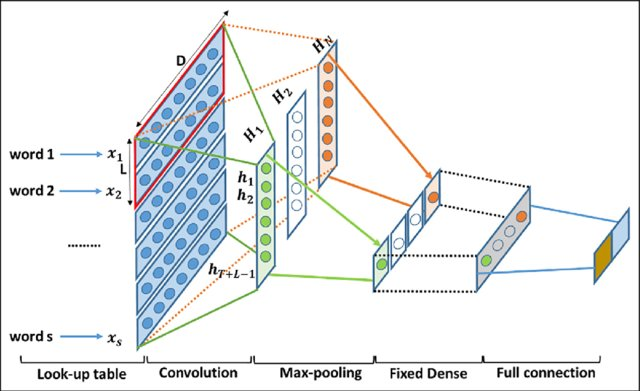
\includegraphics[scale=1.2]{CNN architecture.jpg}
    \caption{CNN architecture}
    \label{fig:cnn artchitecture}
\end{figure}

\begin{description}

    \item[1. Convolutional layer:] The convolutional layer applies convolutional operations to sequential data, such as sentences or documents. The input is typically a matrix where each row represents a word encoded as vector, often using word embeddings like Word2Vec, \ac{glove}. The convolutional layer uses filters (kernels) of various widths that slide over the input text to capture local patterns and n-grams.

    \item[2. Pooling layer:] Pooling layers, such as max pooling, are often used to downsample the feature maps, reducing their dimensionality while retaining the most critical features. For text, max pooling is commonly used to capture the most important feature (e.g., the highest value) from each feature map, regardless of its position.
   
    \item[3. Fully connected layers:] These layers, typically found at the end of the network, connect every neuron in one layer to every neuron in the next layer. They are responsible for combining the extracted features to make the final classification or prediction.
       
\end{description}

\subsection{CNN-LSTM}

Combining \ac{cnn} with \ac{lstm} networks is a powerful technique for handling data with spatial and temporal dependencies. The CNN-LSTM architecture leverages the strengths of both CNNs and LSTMs to handle complex data with spatial and temporal characteristics. The output of the CNN layer (i.e. the feature maps) are the input for the \ac{rnn} layer of LSTM units/cells that follow. The RNN layer uses the local features extracted by the CNN and learns the long-term dependencies of the local features of news articles to classify them as fake or real. The proposed model is depicted in fig \ref{fig:cnn-lstm}. \\

\begin{figure}[h]
    \centering
    
\includegraphics[scale=0.9]{cnn-rnn.png}
    \caption{CNN-LSTM}
    \label{fig:cnn-lstm}
\end{figure}

The LSTM consists of the following control gates :

\begin{description}

    \item[1. Input gate:] The input gate determines which values from the input should be used to modify the memory. It utilizes a sigmoid function to decide which values to let through (ranging from 0 to 1) and a tanh function to assign weights to the values, indicating their level of importance.

    \item[2. Forget gate:] The forget gate determines what information should be discarded from the memory cell. It also employs a sigmoid function, which looks at the previous state and current input, and outputs values between 0 (omit this information) and 1 (keep this information) for each element in the memory cell state.
   
    \item[3. Output gate:] The output gate combines the input and memory of the LSTM block to determine the output. It uses a sigmoid function to decide which values to pass through (ranging from 0 to 1) and a tanh function assigns weights to the values, indicating their level of importance. The weighted values are then multiplied with the output of the sigmoid function to generate the final output.
       
\end{description}

\subsection{CNN-Attention}

Combining \ac{cnn} with attention mechanisms is a powerful approach to enhance the ability of CNNs to focus on the most relevant parts of the input data. Attention mechanisms enable models to focus on the most relevant parts of the input data, dynamically weighting different parts based on their importance.

\begin{description}

    \item[1. Attention layer:] The attention mechanism computes attention scores for the feature maps generated by the CNN. These scores indicate the relevance of each feature in the context of the classification task. The attention mechanism enables the model to focus on the most important parts of the text, enhancing its ability to capture global context and long-range dependencies. The attention scores are used to compute a weighted sum of the feature maps, producing a context vector that represents the most relevant features of the text.
    
\end{description}

\section{Literature Review}

Fake news detection has become an essential area of research due to the rapid spread of misinformation through social media and online news platforms. \ac{cnn}, originally designed for image processing, have shown significant promise in text classification tasks, including fake news detection. This literature review explores key developments, methodologies, and findings in using CNNs for detecting fake news.\\

Yoon Kim's seminal paper applied CNNs to sentence classification tasks. The model used static and dynamic word embeddings, and multiple filter sizes to capture various n-gram features. The study showed that CNNs could capture important local features and patterns in text data, which are crucial for distinguishing between fake and real news \cite{kim2014convolutional}. Wang extended the application of CNNs to fake news detection by training a CNN model on the LIAR dataset. This study highlighted the CNN's ability to learn intricate patterns in the text that are indicative of false or fake news, such as sensational language and specific word usage \cite{wang-2017-liar}. \\

The study \cite{zhang2016characterlevel} proposed using CNNs directly on character-level text, bypassing the need for word embeddings. The model showed that character-level representations could be effective for text classification, especially in cases where word-level information might be sparse or noisy. Conneau and colleagues proposed using very deep CNNs with up to 29 convolutional layers. They demonstrated that deeper networks, along with residual connections, could capture more complex features and improve text classification accuracy \cite{conneau2017deep}.\\

Combining CNNs with RNNs leverages the strengths of both architectures: CNNs for local feature extraction and RNNs for capturing sequential dependencies. Lai et al. introduced a Recurrent Convolutional Neural Network (RCNN) \cite{Lai2015RecurrentCN} for text classification, which improved performance by combining convolutional and recurrent layers.  The research \cite{hybrid-cnn-rnn} shows use of hybrid CNN-RNN model on two fake-news datasets (ISO and FA-KES) with better detection results than other non-hybrid baseline models.\\

Attention mechanisms have been integrated with CNNs to enhance their ability to focus on relevant parts of the text. Yang et al. proposed a Hierarchical Attention Network (HAN) \cite{yang-etal-2016-hierarchical} that applied attention at both word and sentence levels.  Attention mechanisms help in identifying key phrases and sentences that are indicative of fake news. \\

\clearpage
\section{Methodology}

The image below shows the general workflow of CNN model for fake news classification. The process involves several steps, which are described below:

\begin{figure}[h]
    \centering
    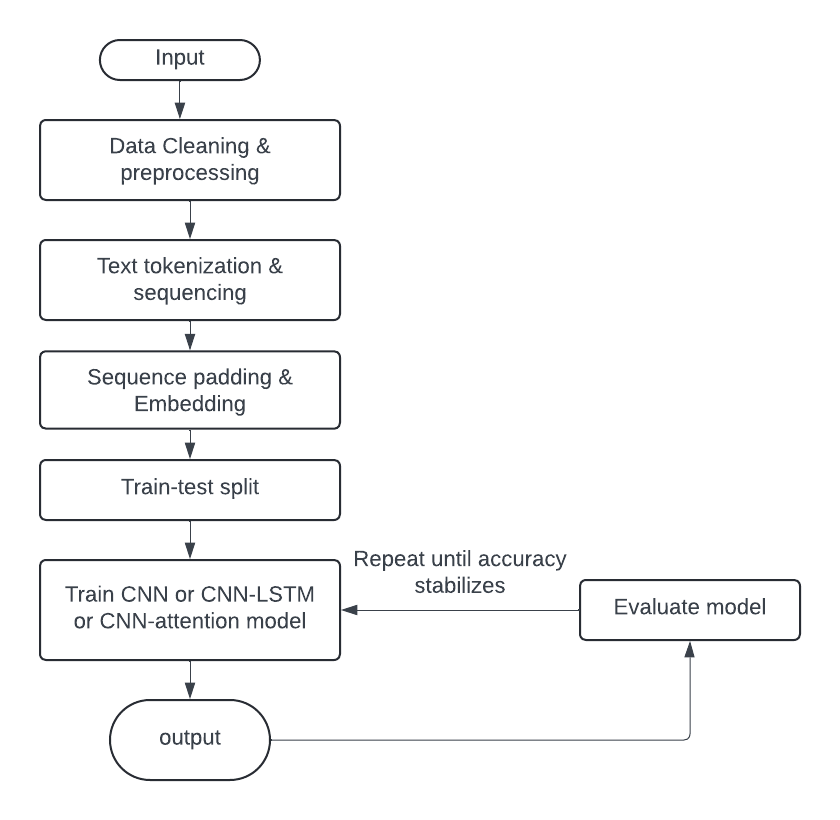
\includegraphics[scale=1.2]{model workflow.png}
    \caption{CNN model workflow}
    \label{fig:cnn workflow}
\end{figure}

\clearpage
\subsection{Dataset Description}

Input Data for this model is taken from kaggle \cite{fake-news-dataset}, an online repository known for its diverse collection of dataset and \ac{ml} competitions. The dataset consists of 20,761 entries, with 10,387 labeled as true news and the remaining 10,374 as fake news. In this research, the text field and label field of the data is used for training the model. The label has 1 for fake news and 0 for true news.

\begin{figure}[h]
    \centering
    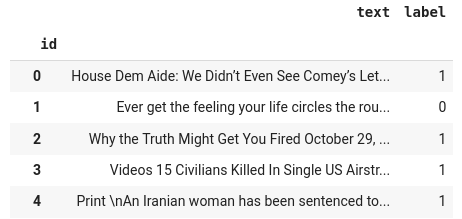
\includegraphics[scale=0.8]{dataset.png}
    \caption{Dataset structure}
    \label{fig:Dataset structure}
\end{figure}

\subsection{Data Cleaning and Preprocessing}

Data cleaning and preprocessing is done to reduce noise or irrelevant information like stopwords. It helps to standardize text by converting it to lowercase, improves performance of model. The input data is passed to a function which converts text to lowercase, remove stopwords, and lemmatize each word. Lemmatization is the process of reducing words to their base or root form, which helps in standardizing words for tasks like text analysis and \ac{nlp}.

\subsection{Tokenization and Sequencing}

To transform the text in each entry before feeding it to the CNN model, the first step is to tokenize words. Tokenization is the process of breaking down text into smaller units called tokens. These tokens can be words, subwords, or characters. The goal of tokenization is to convert raw text into a format that can be numerically processed by a neural network. Once tokenized, the tokens need to be converted into sequences of numerical values that the CNN can process.

\subsection{Padding and Embedding}

Padding is done to ensure all sequences have same length. This is often done by padding shorter sequences with zeros or truncating longer sequences. Embedding in the context of \ac{nlp} refers to the representation of words (or tokens) as dense vectors of real numbers. These vectors capture semantic meanings and relationships between words, enabling the use of words in machine learning models. Embeddings transform words into a numerical form that preserves syntactic and semantic properties, making them suitable for neural networks and other machine learning algorithms. A pretrained \ac{glove} embedding is used. It is an unsupervised learning algorithm for obtaining vector representations for words. Unlike other word embeddings that are based solely on local context, \ac{glove} uses global statistical information from a corpus to produce dense word vectors.

\subsection{Train-Test split}

Dataset is divided into training and testing subsets. Training subset is used to train the model while testing subset is used to evaluate the trained model using metrics like accuracy score, precision, recall etc. 70 percent of dataset is used for training while 30 percent is used for testing. The number of epochs is adjusted during training to assess whether the model is overfitting or underfitting.

\subsection{CNN and It's Variants}
    
    For binary classification problems such as distinguishing between Fake and True news, the mechanisms through which baseline \ac{cnn}, CNN-LSTM, and CNN-Attention models process and classify news text data are elaborated upon here. The focus is on their capability to classify text sequences as either fake or true.

    \subsubsection{\ac{cnn} model}
    \ac{cnn}s are effective at recognizing local patterns in text, such as specific phrases or word combinations, which can be indicative of fake news. It can learn discriminative features from text and can analyze the sentiment of text by detecting overly sensational or biased language often found in fake news. \\
    
    The \ac{cnn} model uses two convolution layer each followed by dropout and max pooling layer. Dropout is used to avoid overfitting. \ac{cnn} captures the spatial pattern on text sequences which are then passed to fully connected layers to perform classification as shown in figure \ref{fig:cnn_model_architecture}. 

    \begin{figure}[h]
        \centering
        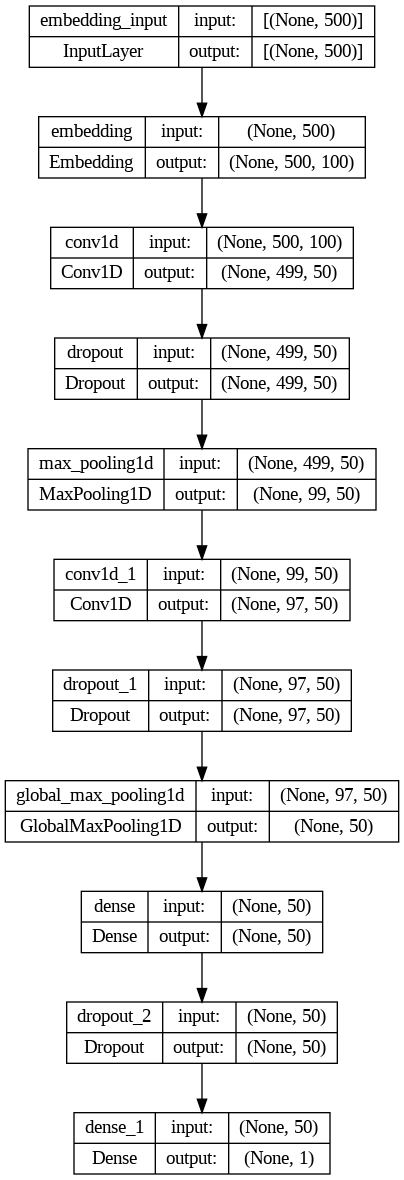
\includegraphics[scale=0.5]{CNN model arch.png}
        \caption{\ac{cnn} model architecture}
        \label{fig:cnn_model_architecture}
    \end{figure}

    \clearpage
    
    \subsubsection{CNN-LSTM model}
    It is a hybrid model which uses \ac{cnn} and \ac{lstm} layers. The pattern detected by \ac{cnn} are passed to \ac{rnn}/\ac{lstm} layer that learns the long-term dependencies of input text. \\

    \ac{lstm}s are designed to capture long-range dependencies in sequences, making them well-suited for understanding context and nuances in news articles. It helps to model the relationship between words and sentences over the entire article making them suitable to use for fake news classification.
    
    \begin{figure}[h]
        \centering
        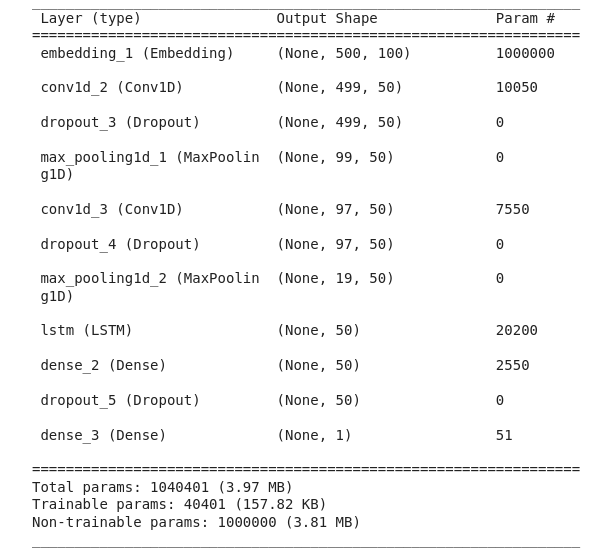
\includegraphics[scale=0.7]{CNN-LSTM-arch.png}
        \caption{CNN-LSTM model architecture}
        \label{fig:cnn-lstm-model-arch}
    \end{figure}

    \clearpage
    \subsubsection{CNN-Attention model}
    It is also a hybrid model which computes attention scores for the data generated by the CNN layer. This hybrid approach leverages the local feature extraction capabilities of CNNs and the context-awareness of attention mechanisms, making it highly effective for tasks like fake news detection.\\

    Attention mechanism calculates attention weights that signify the importance of each word (or feature) in the context of the entire article. It provides contextual information to each feature or word, which is crucial for classifying news as fake or true. The context vector is the weighted sum of the input vectors, with weights determined by the attention mechanism. The attention mechanism itself involves computing intermediate scores using a learned weight matrix W and bias vector b, applying the tanh activation function, and normalizing these scores with the softmax function to obtain the attention weights.

    \[
        \text{context} = \sum_i (\text{softmax}(\tanh(W \cdot x_i + b)) \cdot x_i)
    \]

    \begin{figure}[h]
        \centering
        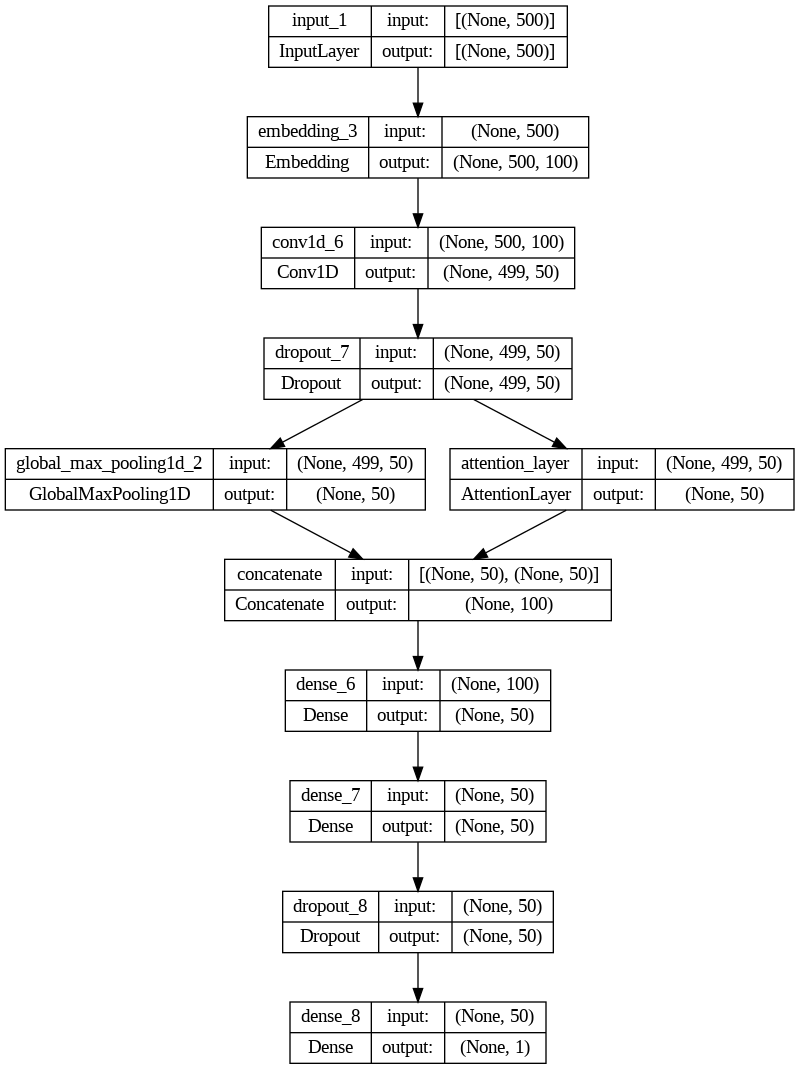
\includegraphics[scale=0.5]{CNN-Attention-arch.png}
        \caption{CNN-Attention model architecture}
        \label{fig:cnn-attention-model-arch}
    \end{figure}

\clearpage
\subsection{Evaluation}

In order to determine the consistency and accuracy of a classification model, typical assessment metrics are determined according to,

\begin{description}
    \item[Accuracy:] Accuracy is the ratio of correctly predicted instances to the total instances. It gives an overall measure of how often the model is correct.
    $$\text{Accuracy} = \frac{\text{True Positives} + \text{True Negatives}}{\text{Total Number of Instances}}$$

    \item[Precision:] Precision (also called Positive Predictive Value) is the ratio of correctly predicted positive observations to total predicted positives. It tells you how many of the instances predicted as positive are actually positive.
    $$ \text{Precision} = \frac{\text{True Positives}}{\text{True Positives} + \text{False Positives}} $$
    
    \item[Recall:]  Recall (also called Sensitivity or True Positive Rate) is the ratio of correctly predicted positive observations to the all observations in the actual class. It tells you how many of the actual positive instances were captured by the model.
    $$ \text{Recall} = \frac{\text{True Positives}}{\text{True Positives} + \text{False Negatives}} $$

    \item[F1 score:] The harmonic mean of recall and precision is the F1 Score. As a result, this score takes both false positives and false negatives into account. F1 score is more useful than accuracy when the class distribution is unbalanced.
    $$ \text{F1 Score} = 2 \times \frac{\text{Precision} \times \text{Recall}}{\text{Precision} + \text{Recall}} $$
\end{description}
\clearpage

\section{Implementation}

\subsection{Implementation Tools}
Python is used as the programming language to code the program. Google Colab is used as an \ac{ide}. Similarly, different libraries are also used as:

\begin{description}
    \item[Tensorflow:] TensorFlow is used to build and train the CNN based Fake News classifier.
    \item[Keras:] Keras is used to simplify the process of building and training the CNN models.
    \item[NLTK:] \ac{nltk} is a powerful library in Python for working with human language data.  It provides easy-to-use interfaces and text processing libraries for classification, tokenization, stemming, tagging, parsing, and more.
    \item[NumPy:] NumPy is used to store and manipulate training and testing data.
    \item[Pandas:] Pandas is used to load and clean training and testing data.
    \item[Matplotlib:] Matplotlib is used to visualize the results of the Fake News classifier.
\end{description}

\subsection{Implementation Details}

\subsubsection{Data Cleaning and Preprocessing} The train and test data are passed through a function which removes stopwords, lowercase, and then lemmatize each word for effective learning of model. The \ac{nltk} library is used to perform data cleaning and preprocessing.

\begin{figure}[h]
    \centering
    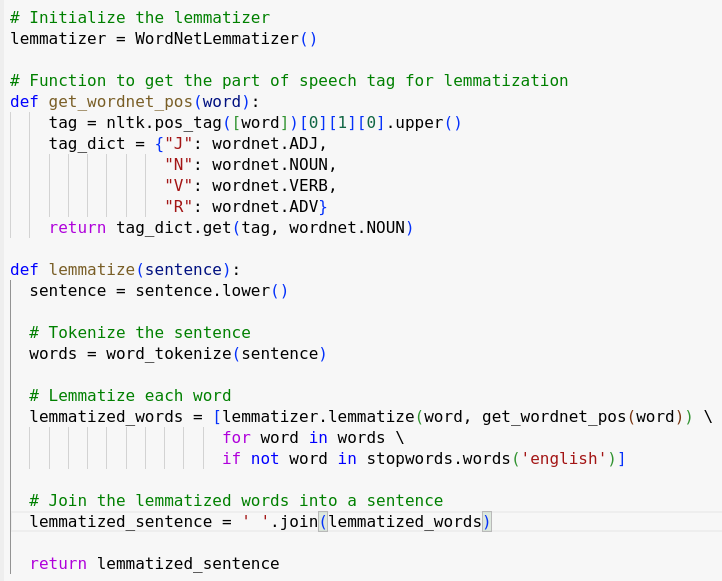
\includegraphics[scale=0.6]{Lemmatization.png}
    \caption{Python code for data cleaning and lemmatization}
    \label{fig:lemmatization}
\end{figure}

\subsubsection{Text Sequencing and Padding} The text data were transformed into sequences of words using a tokenizer, and each sequence was padded with zeros to have a fixed length of 500 words. This step ensured that all sequences had consistent dimensions for efficient processing. The sequence length of 500 words is chosen based on experiment on model's performance.

\begin{figure}[h]
    \centering
    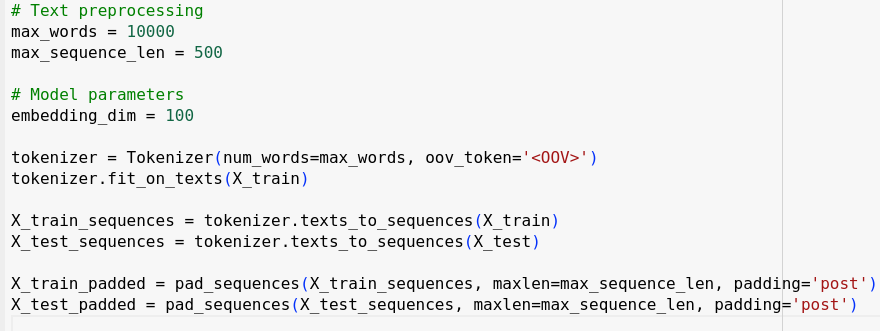
\includegraphics[scale=0.5]{sequencing_and_padding.png}
    \caption{Python code for sequencing and padding text}
    \label{fig:sequencing_and_padding}
\end{figure}

\subsubsection{Embedding} The text sequences are converted to dense 100 dimensional vectors of real numbers using \ac{glove} embedding as shown in figure \ref{fig:embedding_with_glove}. The embeddings are trained on very large text corpora which ensures embeddings generalize well to new unseen text. The pre-trained weights also helps model to train faster without compromising peformance.

\begin{figure}[h]
    \centering
    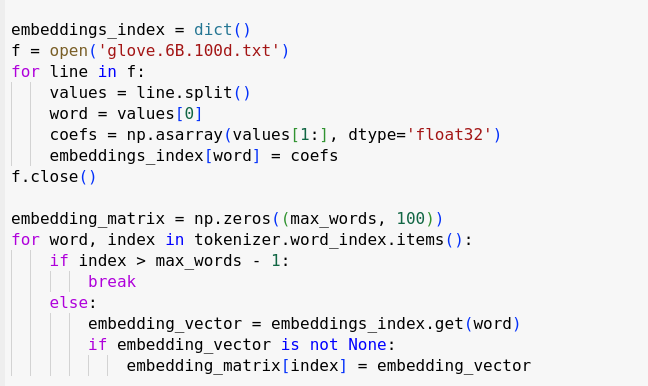
\includegraphics[scale=0.5]{embedding.png}
    \caption{Python code for generating embedding vector with GloVe}
    \label{fig:embedding_with_glove}
\end{figure}

\clearpage
\subsubsection{CNN Architecture}
\subsubsection{Baseline CNN}
The CNN model consists of Embedding layer, two convolutional layers followed by pooling layer. The sequence of words are initially transformed into 100-dimensional vectors through an embedding layer, enhancing the model’s ability to process text input effectively. Dropout is used to combat overfitting in training data, finally the model is passed to dense layer. Convolution layer applies filter and, Pooling layer down-samples feature maps retaining most crucial features only. The model concludes with a softmax-activated dense layer, enabling binary classification.

\begin{figure}[ht]
    \centering
    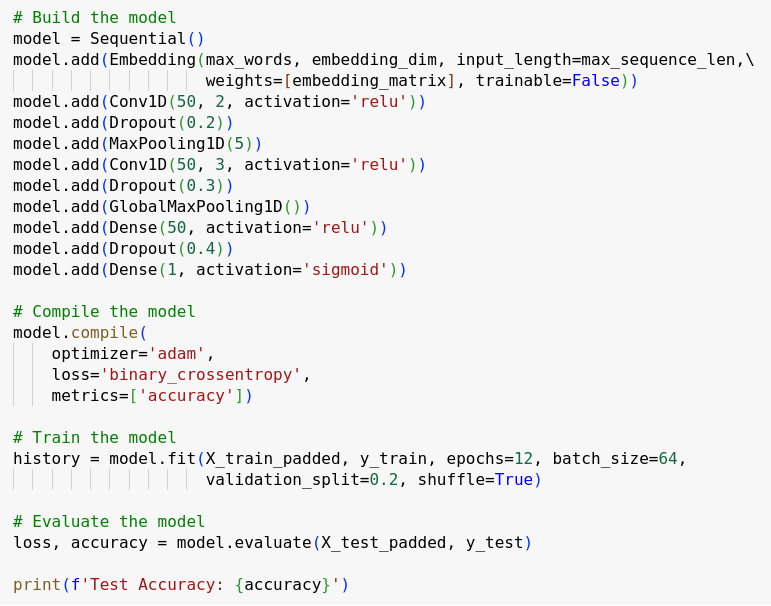
\includegraphics[scale=0.5]{cnn-implementation.png}
    \caption{CNN implementation}
    \label{fig:cnn_implementation}
\end{figure}

\clearpage

\subsubsection{CNN-LSTM}
The CNN-LSTM model uses CNN layers followed by LSTM layers. The CNN layer is similar to classic CNN architecture, LSTM layers consist of 50 units. The LSTM use tanh activation function and sigmoid for recurrent activation.

\begin{figure}[h]
    \centering
    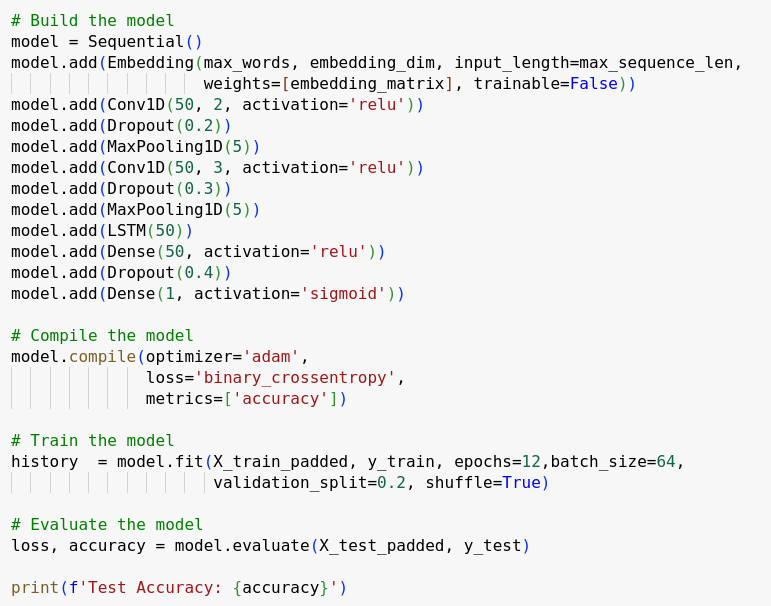
\includegraphics[scale=0.5]{cnn-lstm-implementation.png}
    \caption{CNN-LSTM implementation}
    \label{fig:cnn-lstm-implementation}
\end{figure}

\subsubsection{CNN-Attention}
The CNN-Attention model uses CNN layer followed by an Attention layer. The Attention layer uses output from the preceding CNN layer to computes attention weights and produce a context vector. The code to calculate attention weights is shown in figure \ref{fig:attention-implementation}.

\begin{figure}[h]
    \centering
    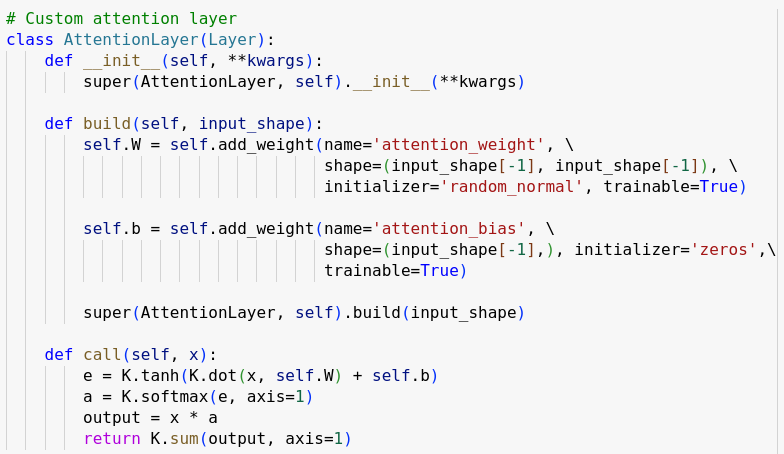
\includegraphics[scale=0.5]{attention_implementation.png}
    \caption{Attention implementation}
    \label{fig:attention-implementation}
\end{figure}

\begin{figure}[h]
    \centering
    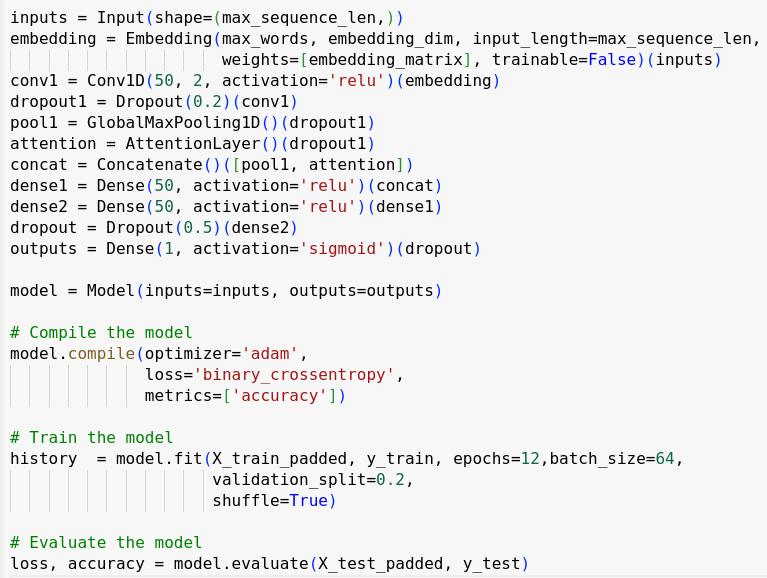
\includegraphics[scale=0.5]{cnn-attention-implementation.png}
    \caption{CNN-Attention implementation}
    \label{fig:cnn-attention-implementation}
\end{figure}

\clearpage
\subsubsection{Model Optimization and Training} 
For model optimization, Adam optimizer and binary cross-entropy loss function was utilized. The evaluation metrics included accuracy, precision, and recall. The models were trained for 12 epochs.

\subsubsection{Model Evaluation} 
The models' performance is assessed using a test dataset by generating categorical predictions through the \lq predict\rq\  method. These predictions are compared to actual labels to form a confusion matrix, from which accuracy, precision, and recall are calculated to evaluate the models' effectiveness in classifying true or fake news.

\begin{figure}[h]
    \centering
    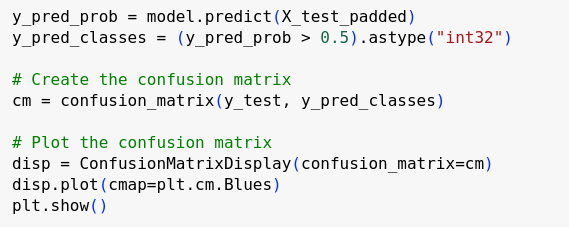
\includegraphics[scale=0.65]{confusiong matrix code.png}
    \caption{Code for confusion matrix}    
\end{figure}

\section{Findings and Result}

\subsection{Confusion Matrix}
The confusion matrix displays the performance evaluation of a classification model on test dataset. It consists of actual classes and predicted classes.

\subsubsection{Confusion matrix of Baseline CNN}

\begin{description}
    \item[True Positives (TP):] There are 2951 true positives, correctly predicting ‘Fake’.
    \item[False Negatives (FN):] There are 161 false negatives, incorrectly predicting ‘Fake’.
    \item[False Positives (FP):] There are 95 false positives, incorrectly predicting 'True'.
    \item[True Negatives (TN): ] There are 2999 true negatives, correctly predicting ‘True’.
\end{description}

\begin{figure}[h]
    \centering
    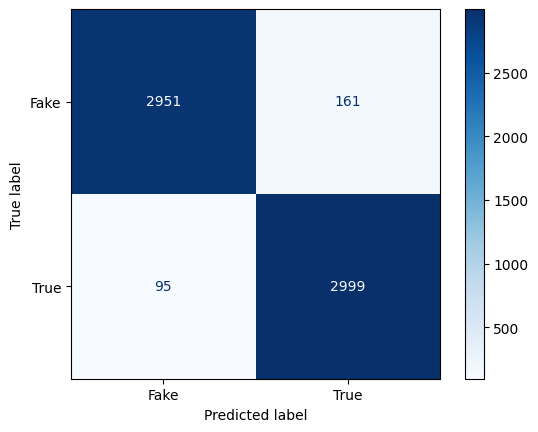
\includegraphics[scale=0.65]{cm_baseline_cnn.png}
    \caption{Confusion matrix of baseline CNN}    
\end{figure}

% \clearpage
\subsubsection{Confusion matrix of CNN-LSTM}

\begin{description}
    \item[True Positives (TP):] There are 3028 true positives, correctly predicting ‘Fake’.
    \item[False Negatives (FN):] There are 84 false negatives, incorrectly predicting ‘Fake’.
    \item[False Positives (FP):] There are 143 false positives, incorrectly predicting 'True'.
    \item[True Negatives (TN): ] There are 2951 true negatives, correctly predicting ‘True’.
\end{description}

\begin{figure}[h]
    \centering
    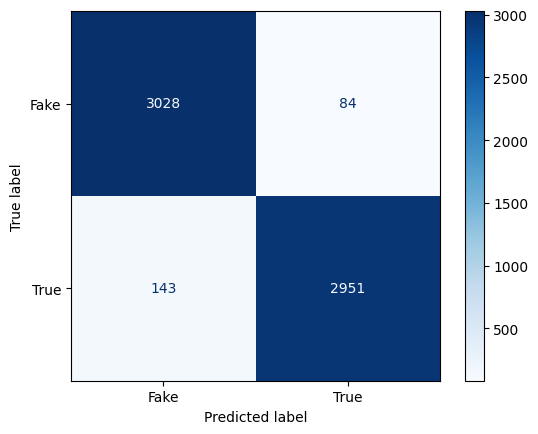
\includegraphics[scale=0.65]{cm_cnn-lstm.png}
    \caption{Confusion matrix of CNN-LSTM}
    \label{fig:cm_cnn-lstm}
\end{figure}
\clearpage
\subsubsection{Confusion matrix of CNN-Attention}

\begin{description}
    \item[True Positives (TP):] There are 3039 true positives, correctly predicting ‘Fake’.
    \item[False Negatives (FN):] There are 73 false negatives, incorrectly predicting ‘Fake’.
    \item[False Positives (FP):] There are 104 false positives, incorrectly predicting 'True'.
    \item[True Negatives (TN): ] There are 2990 true negatives, correctly predicting ‘True’.
\end{description}

\begin{figure}[h]
    \centering
    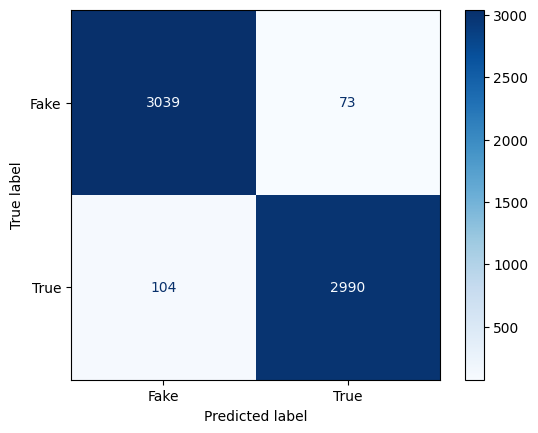
\includegraphics[scale=0.65]{cm_cnn-attention.png}
    \caption{Confusion matrix of CNN-Attention}
    \label{fig:cm_cnn-attention}
\end{figure}


% \clearpage
\subsection{Accuracy Parameters} 
The accuracy parameters using \ac{cnn} variants is evaluated on test dataset. The observations is listed below:

\begin{table}[h]
    \caption{Accuracy parameters of CNN variants}
    \centering
    \begin{tabular}{|c|c|c|c|}
    \hline
      \textbf{Model} & \textbf{CNN} & \textbf{CNN-LSTM} & \textbf{CNN-Attention} \\
      \hline
        \textbf{Accuracy} &95.87\%  &96.34\% & 97.14\%\\
        \hline
        \textbf{Precision} & 96\%& 96\%&97\% \\
        \hline
        \textbf{Recall} & 96\%&96\% &97\% \\
       \hline
       \textbf{F1 score} & 96\%&96\% &97\% \\
       \hline
    \end{tabular} 
   
    \label{tab:accuracy_params_of_cnn_variants}
\end{table}

Comparing \ac{cnn} and it's variants, there is stable precision and recall while precision, recall and accuracy slightly increases for CNN-Attention variant. Based on accuracy parameters CNN-Attention has performed better.
\clearpage

\subsection{Overfitting and Generalization} 
The training and validation loss and accuracy plots demonstrated a smooth convergence throughout the training process, indicating that the model effectively learned from the data without signs of overfitting or underfitting.

\begin{figure}[h]
    \centering
    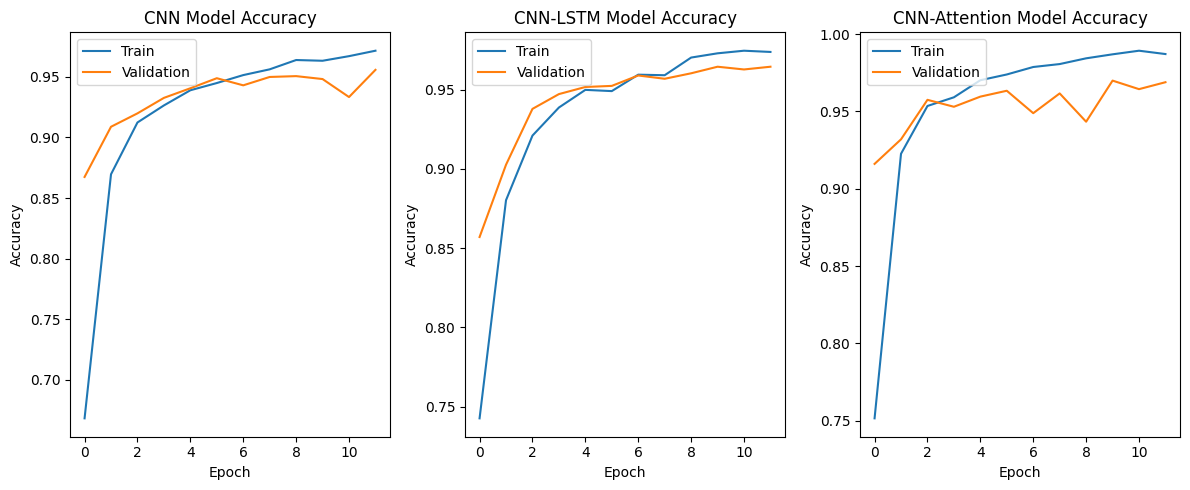
\includegraphics[scale=0.52]{accuracy images.png}
    \caption{Training and validation accuracy over epochs for CNN, CNN-LSTM and CNN-Attention}  
\end{figure}

\begin{figure}[h]
    \centering
    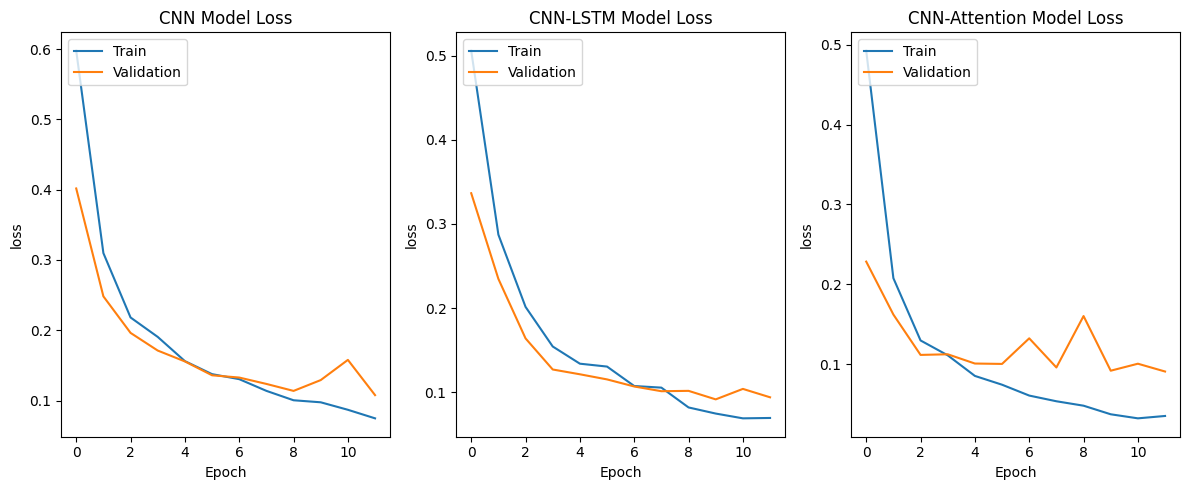
\includegraphics[scale=0.52]{loss images.png}
    \caption{Training and validation loss over epochs for CNN, CNN-LSTM and CNN-Attention}   
\end{figure}
\clearpage
\subsection{Result Analysis}
The accuracy, precision and recall observed on various \ac{cnn} models suggest that the local patterns detected by baseline \ac{cnn} like specific words or phrase combinations is enough for fake news classification. The long-range dependencies by LSTM layer did not increased accuracy by significant amount compared to CNN-Attention model, which suggests long-range dependencies is not much critical or enough for the task on current dataset. Better performance of CNN-Attention, +0.8\% accuracy than CNN-LSTM and +1.3\% accuracy than baseline CNN suggest, focusing on informative parts of the text by dynamically weighing using attention mechanism can enhance model performance. It highlights the fact that adding contextual information to words using attention mechanism is indeed useful. \\

The training and validation accuracy and loss over epoch is similar on all models suggesting, all models are converging to similar level of performance. Model are learning effectively from the data and are not significantly overfitting or underfitting. The models converges at 12\textsuperscript{th} epoch.


    \chapter{Conclusion}

\section{Conclusion}

The study compared the performance of three CNN-based models - baseline CNN, CNN-LSTM, and CNN-Attention - for Fake News classification. Evaluation metrics such as accuracy, precision, recall, and F1 score were used. \\

The CNN-Attention model emerged as the top performer, exhibiting the highest accuracy, precision and recall. Despite a slightly higher count of false positives compared to baseline \ac{cnn}, it demonstrated superior overall performance in accurately classifying `Fake' and `True' news.\\

In conclusion, the CNN-Attention model stands as the optimal choice for Fake News classification tasks, offering superior accuracy, precision and recall with 97.14\% accuracy and 97\% precision and recall on test dataset.

\section{Future Recommendation}

Exploring more recent and advanced \ac{cnn} architectures or hybrid model that combine \ac{cnn} with other neural network structures (e.g, Transformers) could potentially enhance classification accuracy further. Integrating multi-modal data (e.g. text, images, videos) could improve model's ability to understand and detect fake news. Use of cross-lingual datasets could prevent model from biasing toward specific languages or regions. \\

Furthermore, developing and training model on Nepali news texts could improve the detection of fake news in the Nepali language, catering to the local population's needs and enhancing the overall reliability of the model in different linguistic scenarios. This would involve creating or curating a large,  labeled dataset of Nepali news articles, both real and fake.  
    
    \bibliography{references}
    \bibliographystyle{unsrt}
    
    \addcontentsline{toc}{section}{References}
    
\end{document}